% Move red left, easy case: h.right.left is black; one color flip suffices.
% Editable source for this diagram. From this directory, regenerate with:
% latex -interaction=nonstopmode -halt-on-error llrbt-7.tex
% dvisvgm --no-fonts --exact --bbox=papersize --output=llrbt-7.svg llrbt-7.dvi
\documentclass[tikz,border=12pt]{standalone}
\usepackage{lmodern}
\usepackage{tikz}
\usetikzlibrary{arrows.meta,backgrounds,shapes.geometric,patterns}
\definecolor{linkred}{HTML}{B5240A}
\definecolor{noteBlue}{HTML}{0067A5}
\definecolor{softgreen}{HTML}{D8EAD0}
\definecolor{softpurple}{HTML}{D9D1E8}
\definecolor{softpink}{HTML}{F5CECF}
\definecolor{softyellow}{HTML}{FFF2C9}
% Translucent vector layers keep the soft shadow in the DVI-to-SVG export.
\tikzset{
  llrbt shadow layer/.style args={#1/#2}{
    preaction={fill=black,draw=none,fill opacity=#2,
      transform canvas={shift={(3pt,-3pt)},
        scale around=#1:(current path bounding box.center)}}
  },
  llrbt shadow/.style={
    llrbt shadow layer=1.40/0.01,
    llrbt shadow layer=1.35/0.015,
    llrbt shadow layer=1.30/0.025,
    llrbt shadow layer=1.25/0.04,
    llrbt shadow layer=1.20/0.06,
    llrbt shadow layer=1.15/0.08,
    llrbt shadow layer=1.10/0.10,
    llrbt shadow layer=1.05/0.12,
    llrbt shadow layer=1.00/0.14,
    llrbt shadow layer=0.95/0.16,
    llrbt shadow layer=0.90/0.18,
    llrbt shadow layer=0.85/0.20
  }
}
\begin{document}
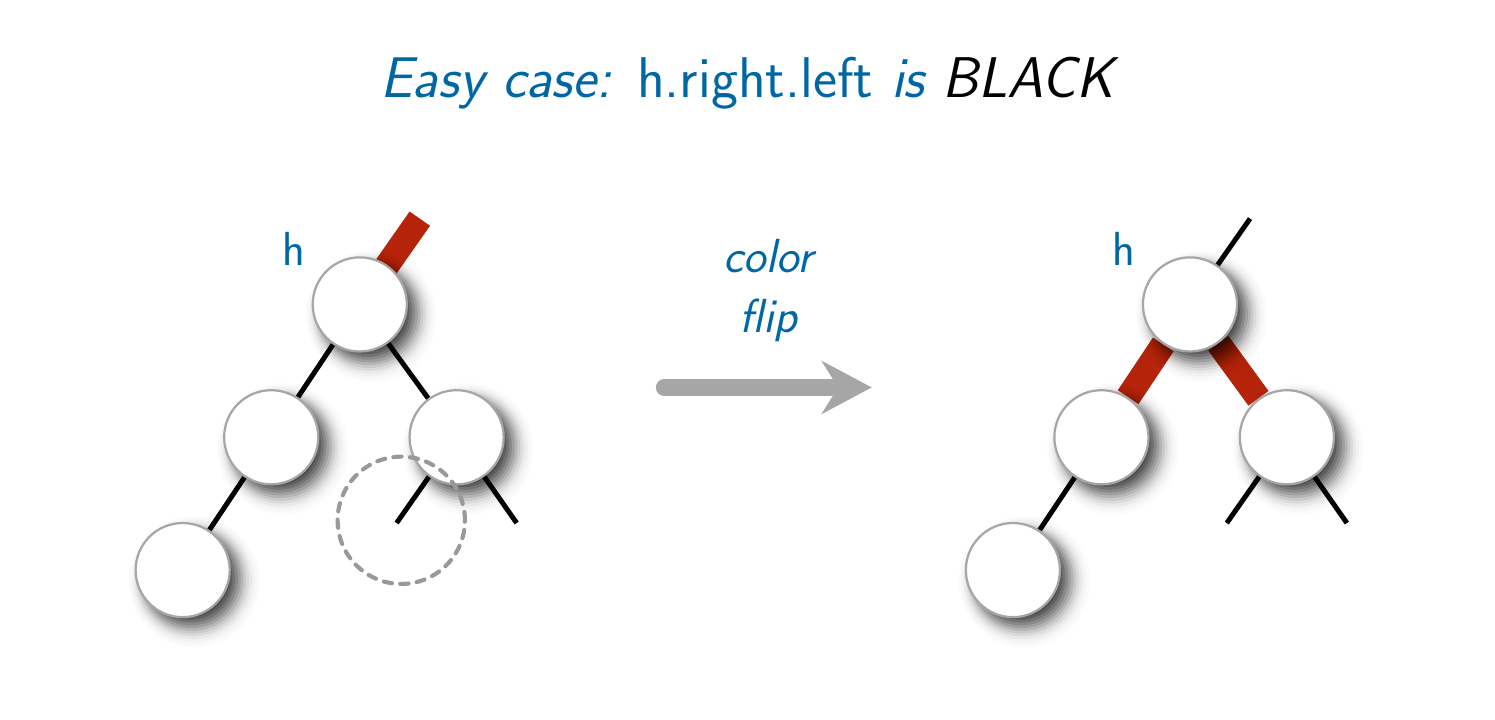
\begin{tikzpicture}[x=1pt,y=-1pt,>=Stealth,line cap=round,line join=round]
\path[use as bounding box] (0,0) rectangle (520,240);
\begin{scope}[on background layer]
\draw[draw=linkred,line width=9pt] (120,100) -- (141.7,69);
\draw[draw=black,line width=1.8pt] (155,148) -- (133.3,179);
\draw[draw=black,line width=1.8pt] (155,148) -- (176.7,179);
\draw[draw=black,line width=1.8pt] (420,100) -- (441.7,69);
\draw[draw=black,line width=1.8pt] (455,148) -- (433.3,179);
\draw[draw=black,line width=1.8pt] (455,148) -- (476.7,179);
\end{scope}
\node[llrbt shadow,circle,draw=black!35,fill=white,text=noteBlue,minimum size=34pt,inner sep=0pt,line width=0.8pt,font=\sffamily\fontsize{18}{21.6}\selectfont,font=\sffamily\itshape\fontsize{18}{22}\selectfont] (ah) at (120,100) {};
\node[llrbt shadow,circle,draw=black!35,fill=white,text=noteBlue,minimum size=34pt,inner sep=0pt,line width=0.8pt,font=\sffamily\fontsize{18}{21.6}\selectfont,font=\sffamily\itshape\fontsize{18}{22}\selectfont] (al) at (88,148) {};
\node[llrbt shadow,circle,draw=black!35,fill=white,text=noteBlue,minimum size=34pt,inner sep=0pt,line width=0.8pt,font=\sffamily\fontsize{18}{21.6}\selectfont,font=\sffamily\itshape\fontsize{18}{22}\selectfont] (ar) at (155,148) {};
\node[llrbt shadow,circle,draw=black!35,fill=white,text=noteBlue,minimum size=34pt,inner sep=0pt,line width=0.8pt,font=\sffamily\fontsize{18}{21.6}\selectfont,font=\sffamily\itshape\fontsize{18}{22}\selectfont] (all) at (56,196) {};
\node[llrbt shadow,circle,draw=black!35,fill=white,text=noteBlue,minimum size=34pt,inner sep=0pt,line width=0.8pt,font=\sffamily\fontsize{18}{21.6}\selectfont,font=\sffamily\itshape\fontsize{18}{22}\selectfont] (bh) at (420,100) {};
\node[llrbt shadow,circle,draw=black!35,fill=white,text=noteBlue,minimum size=34pt,inner sep=0pt,line width=0.8pt,font=\sffamily\fontsize{18}{21.6}\selectfont,font=\sffamily\itshape\fontsize{18}{22}\selectfont] (bl) at (388,148) {};
\node[llrbt shadow,circle,draw=black!35,fill=white,text=noteBlue,minimum size=34pt,inner sep=0pt,line width=0.8pt,font=\sffamily\fontsize{18}{21.6}\selectfont,font=\sffamily\itshape\fontsize{18}{22}\selectfont] (br) at (455,148) {};
\node[llrbt shadow,circle,draw=black!35,fill=white,text=noteBlue,minimum size=34pt,inner sep=0pt,line width=0.8pt,font=\sffamily\fontsize{18}{21.6}\selectfont,font=\sffamily\itshape\fontsize{18}{22}\selectfont] (bll) at (356,196) {};
\begin{scope}[on background layer]
\draw[draw=black,line width=1.8pt] (ah) -- (al);
\draw[draw=black,line width=1.8pt] (ah) -- (ar);
\draw[draw=black,line width=1.8pt] (al) -- (all);
\draw[draw=linkred,line width=9pt] (bh) -- (bl);
\draw[draw=linkred,line width=9pt] (bh) -- (br);
\draw[draw=black,line width=1.8pt] (bl) -- (bll);
\end{scope}
\node[anchor=center,text=noteBlue,font=\sffamily\itshape\fontsize{20}{24}\selectfont] at (260,20) {Easy case: \textup{h.right.left} is \textcolor{black}{BLACK}};
\node[anchor=center,text=noteBlue,font=\sffamily\fontsize{18}{21.6}\selectfont] at (96,80) {h};
\node[anchor=center,text=noteBlue,font=\sffamily\fontsize{18}{21.6}\selectfont] at (396,80) {h};
\draw[draw=black!40,dashed,line width=1.5pt] (135,178) circle (23pt);
\draw[draw=black!35,line width=6pt,->,>={Stealth[length=18pt,width=19pt]}] (230,130) -- (305,130);
\node[anchor=center,text=noteBlue,font=\sffamily\fontsize{18}{21.6}\selectfont,align=center,font=\sffamily\itshape\fontsize{18}{22}\selectfont] at (267.5,95.0) {color\\flip};
\end{tikzpicture}
\end{document}
